%
% Tesi D.S.I. - modello preso da
% Stanford University PhD thesis style -- modifications to the report style
%
%%%%%%%%%%%%%%%%%%%%%%%%%%%%%%%%%%%%%%%%%%%%%%%%%%%%%%%%%%%%%%%%%%%%%%%%%%%
%                                                                         %
%			TESI DOTTORATO                                                   %
%			______________                                                   %
%                                                                         %
%			AUTORE: Elena Pagani                                             %
%                                                                         %
%			Ultima revisione: 7.X.1998                                       %
%                                                                         %
%%%%%%%%%%%%%%%%%%%%%%%%%%%%%%%%%%%%%%%%%%%%%%%%%%%%%%%%%%%%%%%%%%%%%%%%%%%
%
%
\documentclass[12pt]{report}
   %\renewcommand{\baselinestretch}{1.5}      % interline spacing
%
% \includeonly{}
%
%			PREAMBOLO
%

\usepackage[a4paper]{geometry}
\usepackage{amssymb,amsmath,amsthm}
\usepackage{graphicx}
\usepackage{bm}
\usepackage{url}
\usepackage{hyperref}
\usepackage{epsfig}
\usepackage[italian]{babel}
\usepackage{setspace}
\usepackage{tesi}
\usepackage[sorting=none]{biblatex}
\usepackage{algorithm}% http://ctan.org/pkg/algorithms
\usepackage{algpseudocode}%
\usepackage[detect-all]{siunitx} 

\makeatletter
\renewcommand{\ALG@name}{Algoritmo}
\makeatother

% per le accentate
\usepackage[utf8]{inputenc}
%
\newtheorem{myteor}{Teorema}[section]
%
\theoremstyle{definition}
\newtheorem{exmp}{Esempio}[section]

%
\newenvironment{teor}{\begin{myteor}\sl}{\end{myteor}}
\bibliography{references.bib}

%
%
%			TITOLO
%
\begin{document}
\title{Rilevazione di fake news basata sull'induzione di insiemi fuzzy}
\author{Giovanni LAGANÀ}
\dept{Corso di Laurea Magistrale in Informatica}
\anno{2019-2020}
\matricola{928792}
\relatore{Prof. Dario MALCHIODI}
\correlatore{Prof. Alfio FERRARA}
%
%        \submitdate{month year in which submitted to GPO}
%		- date LaTeX'd if omitted
%	\copyrightyear{year degree conferred (next year if submitted in Dec.)}
%		- year LaTeX'd (or next year, in December) if omitted
%	\copyrighttrue or \copyrightfalse
%		- produce or don't produce a copyright page (false by default)
%	\figurespagetrue or \figurespagefalse
%		- produce or don't produce a List of Figures page
%		  (false by default)
%	\tablespagetrue or \tablespagefalse
%		- produce or don't produce a List of Tables page
%		  (false by default)
%
%			DEDICA
%
\beforepreface
        {\hfill \Large {\sl \begin{flushright} Dedica da inserire.         
\end{flushright}         }}
%
%			PREFAZIONE
%
%\prefacesection{Prefazione}
%hkjafgyruet.
%
%%
%%
%%			ORGANIZZAZIONE
%\section*{Organizzazione della tesi}
%\label{organizzazione}
%La tesi \`e organizzata come segue:
%\begin{itemize}
%\item nel Capitolo 1 ....
%\end{itemize}
%
\afterpreface

%
%
%			CAPITOLO 1: 

\chapter*{Introduzione}
\addcontentsline{toc}{chapter}{Introduzione} \markboth{Introduzione}{} 
\onehalfspacing

Prova per citare tutti i libri
\cite{1,2,3,4,5,6,7,8,9,10,11,12,13,14,15,16,17,18,19,20,21,22}


\chapter{Stato dell'arte}
\label{Capitolo 1}
\onehalfspacing

Il Capitolo che apre questo elaborato è inerente allo stato dell'arte. Esso si compone come segue: il Paragrafo \ref{fakenews} descrive il problema delle fake news, menzionando la disciplina del fact-checking; il Paragrafo \ref{nlp} riporta le tecniche di elaborazione del linguaggio naturale, soffermandosi sulla gestione del rumore per la fase di preprocessing, sulla rielaborazione e sull'embedding per convertire tale testo in un dato di tipo numerico.
Il Paragrafo \ref{insiemifuzzy} presenta il concetto degli insiemi fuzzy e fornisce una motivazione del perché essi siano uno strumento adeguato per il problema delle fake news.
Infine, il Paragrafo \ref{induzione} porta alla luce i principali componenti del processo di induzione considerato.

\section{Fake news} \label{fakenews}
L'avvento dei news media e dei social media ha portato a una proliferazione e a un consumo crescenti di notizie.
\\
In generale, la circolazione di notizie su questi canali ha fatto sì che aumentassero esponenzialmente le cosiddette \textit{fake news}.
\\
Per fake news si intendono quelle notizie riportanti fatti che volutamente non corrispondono alla realtà.
In questo senso, si evidenzia la necessità di riconoscere e combattere questo fenomeno con l'obiettivo di contrastare il fomentare dell'odio, un'arma che al giorno d'oggi può essere usata come carburante di diffamazione, lucro, terrorismo e xenofobia.
\\
Il problema di questo tipo di notizie è che possono mischiarsi con tutte le altre, portando il lettore a confondere un fatto realmente accaduto con uno volutamente modificato a proprio vantaggio per un secondo fine.
\\
Inoltre, esiste un'intrinseca difficoltà nel valutare la veridicità di una notizia sia per il problema di attingere a fonti attendibili, sia per la natura stessa del testo scritto.

\subsection{Fact-checking} \label{factchecking}
In generale, al di là di quale sia il secondo fine di chi diffonde fake news, il nemico numero uno del giornalismo è la disinformazione.
Per questo motivo un lavoro da sempre svolto da giornalisti, e non, è quello del \textit{fact-checking}: si tratta di una serie di attività mirate alla verifica accurata e puntuale delle fonti.
Secondo questo criterio, la verifica delle sorgenti di informazione avrebbe il vantaggio di validare i fatti, non lasciando spazio ad avvenimenti non confermati da fonti autorevoli.
\\
Questo approccio, però, presenta delle criticità, ad esempio l'assunzione che una fake news non abbia fonti: esistono notizie che, pur attenendosi alle fonti, possono esaltare aspetti apparentemente secondari o di dettaglio che, se esasperati, possono alterare la narrazione di un fatto, fino a sconvolgerla.
\\
Un altro aspetto è che non è così semplice stabilire con certezza quando una fonte sia autorevole e quando no; inoltre, è opinabile assumere a priori che una fonte considerata autorevole non commetta mai a sua volta errori di questo tipo.
\\
Uno dei problemi maggiori, oltre al fatto che la verifica della veridicità di una notizia richieda del tempo, è che la smentita non finisce mai per avere la stessa risonanza e visibilità della notizia falsa. Questo amplifica l'esigenza di trovare un metodo per prevenire il problema, piuttosto che risolverlo a posteriori.
\\
La necessità di arginare questo fenomeno ha spinto i media, soprattutto tradizionali, a impegnarsi in un costante lavoro di fact-checking, lungo, impegnativo e reso ancora più difficile dal fatto che spesso le varie realtà agiscono in maniera autonoma.
\\
Ci si chiede, quindi, se il progresso in ambito informatico possa contribuire ad arginare il problema in maniera efficace.
\\
In letteratura sono stati fatti vari studi per la cosiddetta automazione del fact-checking \cite{5, 6, 8, 9, 10, 11}; inoltre, in \cite{15, 16, 21} sono stati proposti approcci che, principalmente, si suddividono nelle categorie focalizzate rispettivamente sui metodi \textit{content-based} e \textit{context-based}.
Mentre il primo approccio lavora sul contenuto testuale a livello sintattico, il secondo tenta di estrapolarne il contesto, lavorando a livello semantico.

\section{Elaborazione del linguaggio naturale} \label{nlp}
L'automazione dell'analisi lessicale fa parte dell'ampia branca dell'Informatica che prende il nome di NLP, \textit{Natural Language Processing}, che tra le sue varie declinazioni presenta degli interessanti strumenti per poter estrarre delle feature a partire da dati testuali come le notizie.


\subsection{Tecniche di gestione del rumore} \label{clean}
Come nella stragrande maggioranza dei dataset, anche in quelli testuali è presente del rumore, sia a ``basso livello'' nel contenuto dell'informazione, sia ad ``alto livello'' nella forma dei dati che si sta utilizzando.
\\
Possono essere molte le motivazioni che portano un dataset a presentare errori, anomalie o rumore al suo interno: 
nel caso di osservazioni raccolte manualmente può verificarsi una componente di errore umano; dualmente, dataset generati automaticamente (ad esempio tramite dati raccolti da sensori) possono presentare delle anomalie e produrre risultati imprevisti.
\\
Nel caso dei dati trattati in questo elaborato, inoltre, si ha a che fare con informazioni provenienti dal Web, dunque esiste una maggior probabilità di incontrare osservazioni di natura digitale ricavate da pagine HTML o, addirittura, influenzate dal tipo di codifica scelto per rappresentare caratteri speciali.
\\
In tal senso esistono numerose tecniche per gestire il rumore e, seguendo la distinzione fatta all'inizio di questo Paragrafo, è possibile elencare alcune di esse.
\\
\\
Ad \textit{alto livello} si gestisce la presenza di:
\begin{itemize}
    \item valori mancanti,
    \item osservazioni duplicate,
    \item osservazioni vuote,
\end{itemize}

mentre a \textit{basso livello}, tipicamente, si riscontrano:
\begin{itemize}
    \item caratteri speciali,
    \item URL,
    \item parole contenenti numeri,
    \item punteggiatura,
\end{itemize}

e altri numerosi casi che potrebbero essere aggiunti a questo elenco.
\subsection{Tecniche per rielaborare il testo}
Esistono delle tecniche per riadattare il testo in una forma più conveniente per sua la successiva elaborazione da parte di algoritmi di Machine Learning.
\\
Vari studi nel campo dell'Information Retrieval \cite{22}, infatti, hanno dimostrato che tecniche come lo \textit{stemming}, la \textit{lemmatizzazione} e la rimozione delle cosiddette \textit{stop word} possono migliorare sensibilmente i risultati ottenuti da tali modelli.

\paragraph{Stemming} Lo stemming consiste nell'individuare e rimuovere il suffisso delle parole, in modo da ricavarne la radice, ne viene mostrato un esempio in Tabella \ref{stemming}.
\begin{table}[!h]
\centering
 \begin{tabular}{|c|c|c|} 
 \hline 
 \textbf{Forma} & \textbf{Suffisso} & \textbf{Radice}
\\ [0.5ex] 
\hline
pront\textbf{o} & \textbf{-o} & \textbf{pront} \\
pronunc\textbf{erà} & \textbf{-erà} & \textbf{pronunc} \\
pronunc\textbf{ia} & \textbf{-ia} & \textbf{pronunc} \\
 \hline
\end{tabular}
\caption{Esempio di stemming}
\label{stemming}
\end{table}

\paragraph{Lemmatizzazione} La lemmatizzazione prende in considerazione l'analisi morfologica delle parole ricorrendo a dettagliati dizionari che l'algoritmo utilizza per ottenere il lemma associato.
Un esempio di questa tecnica viene mostrato in Tabella \ref{lemmatization}.
\begin{table}[!h]
\centering
 \begin{tabular}{|c|c|c|} 
 \hline 
 \textbf{Forma} & \textbf{Informazione morfologica} & \textbf{Lemma}
\\ [0.5ex] 
\hline
ragazze & femminile plurale di \textbf{ragazzo} & \textbf{ragazzo} \\
studia & terza persona singolare, presente del verbo \textbf{studiare} & \textbf{studiare} \\
studiando & gerundio del verbo \textbf{studiare} & \textbf{studiare} \\
 \hline
\end{tabular}
\caption{Esempio di lemmatizzazione}
\label{lemmatization}
\end{table}

\paragraph{Rimozione delle stop word}
Gli articoli, le proposizioni, le congiunzioni o gli aggettivi sono esempi tipici di stop word. Queste parole hanno solitamente un'alta frequenza nei documenti ma non aggiungono alcun valore semantico al testo, in quanto sono tipicamente necessarie per la grammatica del linguaggio; pertanto, rimuoverle è una soluzione che viene spesso adottata per ridurre il carico computazionale.
\\
\\
Naturalmente, le considerazioni fatte per queste tre tecniche valgono per qualsiasi lingua.

\subsection{Tecniche di embedding} \label{embedding}
Gli algoritmi di Machine Learning vengono eseguiti per generare dei modelli che sono in grado di fare delle predizioni. Tuttavia, sia i modelli che gli algoritmi in questione necessitano di un input numerico; dal momento che l'obiettivo di questo elaborato è trattare le notizie, cioè un dato tipo di testuale, è fondamentale ricorrere a delle tecniche per produrre una rappresentazione quantitativa delle notizie.
\\
In questo senso, le tecniche di embedding intervengono proprio per trasformare il dato testuale in dato numerico.
Concretamente, questo equivale a trovare una rappresentazione numerica del testo, estraendo delle feature.
\\
Due famose tecniche di embedding sono Word2Vec e Doc2Vec, il cui meccanismo viene illustrato nei paragrafi che seguono.
\subsubsection{Word2Vec} \label{w2v}
Word2Vec è un algoritmo che ha l'obiettivo di trasformare le parole in vettori numerici all'interno di uno spazio  di dimensione prefissata \cite{3}.
Un corpus è composto da documenti, e ogni documento è composto da parole; ciascuna di queste parole, tramite Word2Vec, viene trasformata in un vettore di lunghezza $r$, dove $r$ indica il numero di feature numeriche che vengono considerate. 
\\
Word2Vec si basa sull'utilizzo di reti neurali \cite{3} ed è principalmente implementato tramite due modelli: Skip-Gram e CBOW (Continuous Bag of Words) che vengono descritti qui di seguito.
\\
Per entrambi i modelli l'input è un corpus di documenti, le cui parole vengono distinte in \textit{token}; ciascun token viene codificato con una rappresentazione one-hot\footnote{La codifica one-hot è un processo che viene applicato ai dati categoriali per convertirli in una rappresentazione vettoriale binaria da utilizzare negli algoritmi di apprendimento automatico. In questo caso i dati categoriali sono le parole e ciascuna può essere rappresentata come il vettore binario di tutti i termini presenti nel documento. Se $n$ è il numero di parole, allora il vettore sarà composto da $n-1$ zeri e da un uno, a indicare quale token venga effettivamente rappresentato}.
\\
Per differenziare le due soluzioni, è necessario introdurre il concetto di contesto, poiché Skip-Gram e CBOW lavorano in due direzioni speculari:
mentre la prima si pone l'obiettivo di predire le parole di contesto a partire dal token corrente, la seconda ha lo scopo di predire il token corrente da una finestra di parole di contesto.
\\
Quando una parola $P$ appare in un testo, il suo contesto è quel set di parole che gli appaiono accanto, data una finestra di analisi precedentemente impostata. I molteplici contesti in cui la parola $P$ viene utilizzata servono a costruire una rappresentazione dell’uso di $P$.
\\
Ogni parola viene associata a un vettore denso, ossia una scala di valori numerici vettoriali, il quale è a sua volta messo in associazione con vettori di parole che appaiono in contesti simili, costruendo quelli che vengono definiti \textit{word vectors}.

\paragraph{Skip-Gram}
Si stabilisce una finestra di dimensione $m$ e si scorre ogni token andando a vedere i termini in prossimità, osservando quelli all'interno del raggio $m$.
\\
\begin{figure}
    \centering
    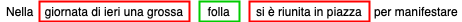
\includegraphics[scale = 0.7]{images/skip-gram.png}
    \caption{Esempio di Skip Gram: in verde il token corrente, in rosso la finestra di contesto grande 5 token}
    \label{skipgram}
\end{figure}
\\
Per esempio, come illustrato in Figura \ref{skipgram}, se \textit{folla} è il token corrente, con $m = 5$ il confronto avviene con \{\textit{giornata}, \textit{di}, \textit{ieri}, \textit{una}, \textit{grossa}, \textit{si}, \textit{è}, \textit{riunita}, \textit{in}, \textit{piazza}\}.
\\
L'idea è quella di cercare di costruire il mapping tra $X$, i token correnti (es: \textit{folla}), e $y$, i token estratti dalla finestra di contesto (es: \textit{piazza}).
\\
Seguendo la notazione tipica di un problema di apprendimento supervisionato, i token presi dalla finestra di contesto sono la variabile target da predire, apprendendo il tipo di relazione che sussiste tra  $X$ e $y$.
\\
Per farlo, come accennato in precedenza, si utilizza una rete neurale, passando la rappresentazione one-hot del dato a un'unità softmax\footnote{Softmax è una possibile funzione di attivazione dello strato di output della rete neurale. In realtà, vale la pena menzionare altre due varianti di criteri di addestramento applicabili, come Negative sampling e Hierarchical Softmax, con diverse implicazioni riguardo efficienza e onere computazionale.}, una funzione che permette di calcolare la probabilità di ottenere una data classe possibile in una serie di modelli di classificazione multi-classe. Per minimizzare una funzione di perdita, che tipicamente è l'entropia incrociata, si utilizza il metodo del gradiente discendente. 

\paragraph{CBOW}
Dualmente a Skip-Gram, CBOW si occupa di predire il token corrente a partire dalla finestra di contesto.
\\
Come mostrato in Figura \ref{cbow}, si predice con quale probabilità si ottenga il token \textit{folla} a partire dalla finestra \{\textit{giornata}, \textit{di}, \textit{ieri}, \textit{una}, \textit{grossa}, \textit{si}, \textit{è}, \textit{riunita}, \textit{in}, \textit{piazza}\}.
\\
\begin{figure}
    \centering
    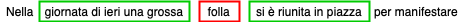
\includegraphics[scale = 0.7]{images/cbow.png}
    \caption{Esempio di CBOW: in rosso il token corrente, in verde la finestra di contesto grande 5 token}
    \label{cbow}
\end{figure}
\\
Anche in questo caso viene addestrata una rete neurale utilizzando il metodo del gradiente discendente per ottenere l'embedding.
\\
\\
In generale, data la natura di queste tecniche, per ottenere una rappresentazione compatta dell'intero documento si rende necessario l'utilizzo in una seconda fase di una tecnica di aggregazione.
\\
In questa fase ogni documento è formato da $n$ parole ed è composto da $n$ vettori lunghi $r$ feature. L'aggregazione interviene per comprimere ciascuno di questi vettori in un valore che sia rappresentativo della corrispondente parola, ottenendo così un vettore per il documento.
\\
Così come in tante altre applicazioni dell'Informatica, i metodi di aggregazione sono molteplici, ad esempio la media aritmetica, la mediana, l'aggregazione del kernel di Fisher \cite{19}.
\\
Fare la media tra vettori significa poter agire su due dimensioni, la prima prevede di sommare prima gli elementi di ciascun vettore e poi dividere per il numero di elementi, ottenendo $n$ valori medi. In realtà, questa soluzione è scomoda per la successiva elaborazione dei dati, dal momento che ogni documento può avere un numero variabile di parole e dunque si otterrebbero vettori di lunghezza diversa per il corpus finale.
\\
La soluzione utilizzata, invece, si applica sommando i primi elementi di tutti i vettori, i secondi, i terzi e così via, per poi dividere per il numero di parole. Così facendo si preserva la rappresentazione tramite feature, perchè si ottiene per ogni documento un vettore lungo $r$; un discorso analogo vale per la mediana.
\\
L'aggregazione del kernel di Fisher, invece, propone una rappresentazione che si basa su quanto il vettore osservato si discosti dal modello generativo GMM (Gaussian Mixture Model). Tale discostamento è una misura di distanza che viene calcolata tramite il gradiente di una funzione di verosomiglianza; i vettori ottenuti prendono il nome di \textit{Fisher vectors}.

\subsubsection{Doc2Vec} \label{d2v}
Doc2Vec nasce come evoluzione di Word2Vec: in questo caso, anziché lavorare a livello di ogni singola parola, si determina direttamente una rappresentazione vettoriale per l'intero documento \cite{24}.
\\
Questo comporta chiaramente il raggiungimento del risultato senza ricorrere a un metodo di aggregazione dei valori.
\\
Conosciuto anche come \textit{Paragraph Vector}, Doc2Vec si articola in due principali implementazioni: PV-DM (Distributed Memory) e DBOW (Distributed Bag of Words).

\paragraph{PV-DM} 
Come per Word2Vec, il task che viene fatto ripetutamente è quello di predire la parola successiva nella frase. I vettori delle parole e i vettori dei paragrafi sono chiamati a contribuire a tale predizione.
\\
Ogni paragrafo viene mappato in un vettore, rappresentato da una colonna nella matrice $D$, così come il vettore di ogni parola è rappresentato da una colonna della matrice $W$ (Figura \ref{pvdm}). I vettori menzionati vengono mediati o concatenati e, a loro volta, essi vengono passati alla rete neurale per prevedere la parola centrale.
\\
La rappresentazione del paragrafo è ciò che effettivamente distingue questa tecnica da Word2Vec, in quanto, pur agendo come un'altra parola, svolge il ruolo di memoria per ricordare cosa manca al contesto corrente; da qui, il nome \textit{Distributed Memory}.
\\
\begin{figure}
    \centering
    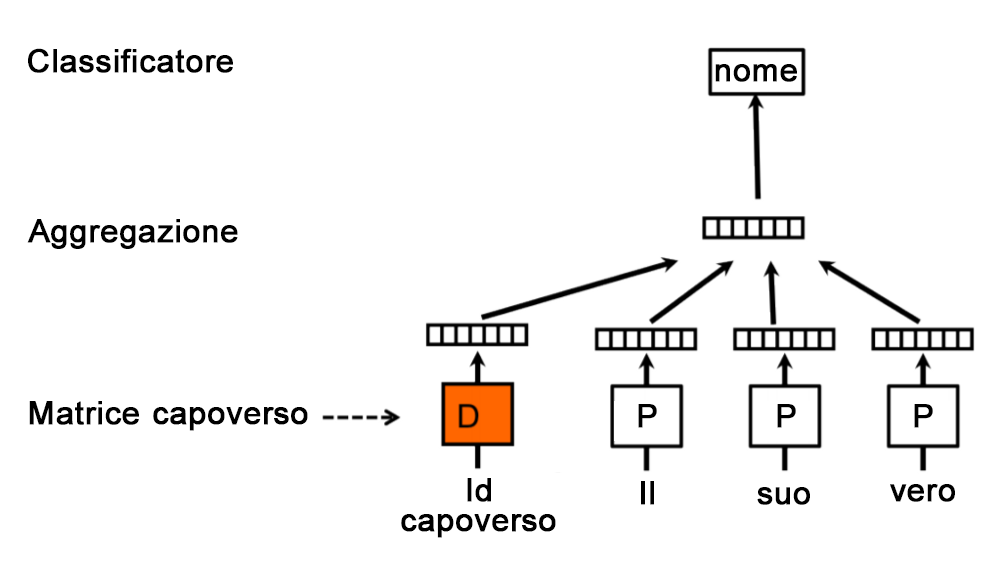
\includegraphics[scale = 0.3]{images/pvdm.png}
    \caption{Architettura in PV-DM (D è la matrice dei documenti e P la matrice delle parole)}
    \label{pvdm}
\end{figure}
\\
La matrice del paragrafo ha, infatti, gli embedding per i paragrafi ``visti'', allo stesso modo in cui i modelli Word2Vec apprendono gli embedding per le parole. Per i paragrafi non visualizzati, invece, il modello viene nuovamente eseguito più volte attraverso la discesa del gradiente per generare un vettore del documento. 

\paragraph{DBOW}
L'architettura DBOW non utilizza le parole di contesto ma effettua la predizione direttamente dalle parole campionate dal paragrafo.
\\
\begin{figure}
    \centering
    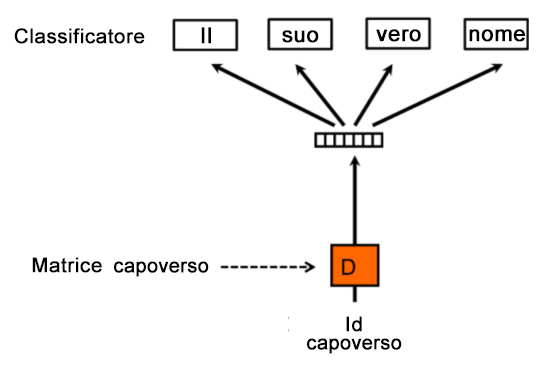
\includegraphics[scale = 0.45]{images/dbow.png}
    \caption{Architettura in DBOW}
    \label{dbow}
\end{figure}
\\
Ne risulta un'architettura (Figura \ref{dbow}) simile a PV-DM ma con il primo livello costituito unicamente dalla matrice dei paragrafi.

\section{Insiemi fuzzy} \label{insiemifuzzy}
Dal momento che questo elaborato si pone l'obiettivo di analizzare le notizie e, nello specifico, di valutare un criterio per individuare quelle fake, è importante introdurre il concetto degli \textit{insiemi fuzzy}.
\\
Diversamente da quanto accade per gli insiemi classici, in cui l'appartenenza  è un concetto binario che viene espresso da un valore di verità, negli insiemi fuzzy esso viene quantificato da un valore continuo tra 0 e 1
\\
Tale valore prende diversi nomi, come \textit{grado di verità} o di \textit{grado di appartenenza}.
\\
In altre parole, gli insiemi fuzzy introducono un significato associato all'appartenenza a un insieme che è più granulare rispetto alla tradizionale dicotomia binaria degli insiemi classici, ottenendo valori che indicano anche se l'espressione sia molto vera, poco vera o mediamente vera.
\\
Nel campo della Sentiment Analysis \cite{25}, per esempio, cercare di determinare le emozioni contenute in un testo rientra in questo tipo di problemi; sarebbe limitante, infatti, considerare unicamente se un tweet o un post esprima felicità o meno, oppure se sia vero o falso che ci sia rabbia nelle parole del messaggio di una persona.
\\
Più realisticamente, esistono componenti più o meno forti di ciascuna di queste emozioni che si mischiano e che formano, complessivamente, un testo.
\\
Tali misture, inoltre, spesso causano dell'incertezza che, di fatto, è la ragione per cui il problema risulta più complesso e, allo stesso tempo, affascinante.
\\
Vari studi, inoltre, hanno evidenziato come l'ambiguità sia una caratteristica intrinseca del linguaggio umano \cite{26, 27}.
Rimanendo nell'esempio della Sentiment Analysis, la presenza di testi con emozioni ambigue è oggi oggetto di ricerca.
\\
Alla luce di tutto ciò, questo elaborato propone di modellare il problema della rilevazione delle fake news come un problema fuzzy, assumendo che le notizie siano associate a insiemi di questo tipo.
\\
L'obiettivo è quello di ricavare un modello di apprendimento supervisionato in grado di produrre il grado di appartenenza a tale insieme, con l'ambizione finale di ottenere un punteggio di affidabilità per ogni notizia;
potenzialmente, tale punteggio rappresenta quanto la notizia sia fake.

\section{Induzione di funzioni di appartenenza} \label{induzione}
In letteratura è stato proposto un algoritmo che fa utilizzo di una procedura originariamente nata come tecnica di support vector clustering per poter indurre la funzione di appartenenza dei punti a un certo insieme fuzzy \cite{1}.
\\
I punti fondamentali di questo approccio riguardano determinare la forma dell'insieme fuzzy e inferire i parametri della sua funzione di appartenenza.

\subsection{Funzione di appartenenza} \label{membership}
Il concetto di funzione di appartenenza si colloca nella teoria degli insiemi e corrisponde alla funzione caratteristica di un insieme.
\\
Fissando l'insieme $A$ e lo spazio $X$, la sua funzione di appartenenza $\mu_A$ tale che $Dom(\mu_A) = X$ è definita come:
\begin{center}
    $\mu_A(x)= \begin{cases} 1 & \mbox{se } x \in A, \\ 0 & \mbox{altrimenti.} \end{cases}$
\end{center}

Secondo la teoria classica degli insiemi, infatti, un insieme è definito come qualunque aggregato (o collezione) di oggetti per il quale sia sempre possibile decidere se un generico oggetto appartiene oppure no all'aggregato stesso\footnote{In realtà, questa definizione è stata dimostrata come fallace verso la fine dell'800, con quella che venne definita la \textit{crisi dei fondamenti della matematica}. Tale crisi produsse una serie di paradossi, tra cui il famoso \textit{paradosso di Russell}, da cui venne derivato il \textit{paradosso del barbiere}. Per rigorosità, sarebbe più opportuno usare una definizione assiomatica degli insiemi, tuttavia al fine di non rendere prolisso il richiamo alla notazione insiemistica classica, è stata preferita una definizione informale.}.
\\
Quando la funzione di appartenenza è booleana, perché si basa su due soli possibili valori (0 o 1), si parla di insieme \textit{crisp}.
\\
Nell'ambito delle notizie, questo corrisponderebbe a classificare ogni notizia come completamente fake o no, a seconda del fatto che appartenga all'insieme.
\\
Lo scopo di questo lavoro, invece, è di rappresentare lo stesso concetto ma in maniera sfumata, producendo informazioni su \textit{quanto} una notizia sia falsa.
\\
Tale rappresentazione ha il vantaggio di poter indicare se una notizia sia più o meno fake di un'altra.
\\
Per questa ragione si introduce il concetto di \textit{grado di appartenenza}, sull'idea di base che il confine di oggetti appartenenti o non appartenenti all'insieme non sia così ben definito.
\\
Ci si concentra, quindi, su una funzione di appartenenza $\mu_A: X \rightarrow [0,1]$ che associa a ogni elemento dell'universo considerato un numero reale compreso tra 0 e 1, dove $X$ è il dominio di $\mu_A$.
\\
Formalmente, si può asserire che:
\begin{itemize}
    \item se $\mu_A(x) = 1$ allora $x$ appartiene all'insieme $A$,
    \item se $\mu_A(x) = 0$ allora $x$ non appartiene all'insieme $A$,
    \item se $0 < \mu_A(x) < 1$ allora $x$ appartiene parzialmente ad $A$ con grado espresso da $\mu_A(x)$.
\end{itemize}

Esempi di concetti fuzzy sono \textit{giovane}, \textit{ricco}, \textit{alto}, mentre non lo sono \textit{fratello}, \textit{studente}, \textit{professore}.
\\
Per determinare il valore di $\mu_A$ vengono definiti diversi tipi di funzioni di appartenenza: funzione sigma, funzione triangolare, trapezoidale, S-Shape, e altre ancora (Figura \ref{membership_functions}). 
\\
\begin{figure}
    \centering
    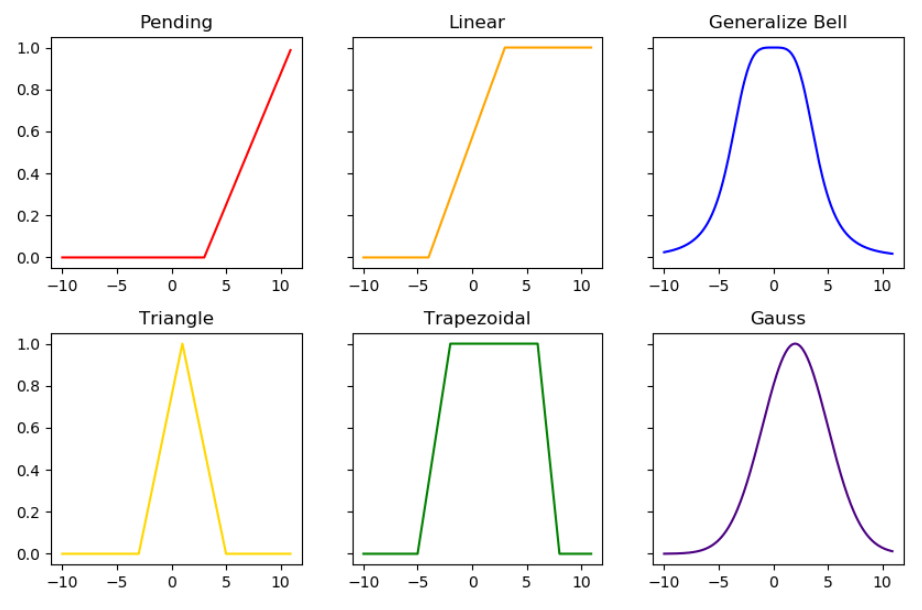
\includegraphics[scale = 0.7]{images/membership_functions.png}
    \caption{Alcuni tipi diffusi di funzioni di appartenenza - da \cite{30}}
    \label{membership_functions}
\end{figure}

\subsection{Metodi kernel} \label{kernel}
La funzione kernel è un oggetto matematico ampiamente utilizzato in congiunzione con le support vector machine \cite{28} anche per problemi di natura non lineare, tuttavia è applicabile anche a numerosi altri contesti, ad esempio la kernel Principal Component Analysis \cite{29}.
\\
Questa metodologia prende il nome di \textit{kernel trick} e consiste nel mappare i punti dallo spazio originale a uno spazio a dimensionalità superiore o infinita, dove il problema diventa lineare.
\\
Tale tecnica si appoggia a una funzione kernel, una funzione simmetrica 
\begin{center}
    $k: \mathcal{X} \times \mathcal{X} \rightarrow \mathbb{R}$
\end{center} 
tale che esistono uno spazio lineare $\mathcal{H}$, detto \textit{spazio delle feature}, in cui è definito un prodotto scalare $<$ ·, · $>$ e una funzione $\mathit{\Phi }: \mathcal{X} \rightarrow \mathcal{H}$ per cui:
\begin{center}
    $k(x,y) = < \mathit{\Phi}(x), \mathit{\Phi}(y) >$ dove $x \in \mathcal{X}$ e $y \in \{-1,1\}$.
\end{center}
I dati vengono, quindi, rappresentati tramite dei confronti di coppie, misurando l'equivalente di una misura di similarità: all'aumentare di $k(x,y)$, $x$ e $y$ sono da considerarsi maggiormente  ``simili''.
\\
Inoltre, tramite l'utilizzo di questo metodo, la dimensionalità dei dati dipende solo dal numero di oggetti e non dalla loro dimensione vettoriale.
\\
Esistono diversi tipi di kernel, ad esempio lineare, polinomiale, iperbolico, gaussiano e molti altri ancora.

\chapter{Soluzione proposta}
\label{Capitolo 2}
\onehalfspacing
Il secondo Capitolo presenta la soluzione che viene proposta in questo elaborato.
Tale soluzione consiste in un sistema di apprendimento supervisionato a partire dall'algoritmo $\bm{\mu}$\textbf{-learn} \cite{1}, il cui funzionamento viene descritto nel Paragrafo \ref{mulearn}.
\\
Nel Paragrafo \ref{sistema}, invece, si mostra l'utilizzo che è stato fatto del presente algoritmo all'interno del sistema, delineando le fasi che si susseguono nel corso degli esperimenti.

\section[\texorpdfstring{L'algoritmo $\mu$-learn}%
                        {mu-learn}]% % choose text-only material here
        {L'algoritmo $\bm{\mu}$-learn}  % note use of \bm ("bold math")
\label{mulearn}
$\mu$-\textit{learn} è un algoritmo di Machine Learning che utilizza una procedura originariamente nata nel contesto del support vector clustering \cite{23}.
\\
Essa si colloca nel gruppo di tecniche che lavora su insiemi fuzzy triangolari, trattando un problema di ottimizzazione non lineare.
\\
La natura di questo problema si rivela conveniente per la diversificazione delle funzioni di appartenenza, i cui parametri vanno a determinare la forma degli insiemi fuzzy formati.
\\
Il nome di questo algoritmo suggerisce il suo obiettivo: apprendere $\mu$, la funzione di appartenenza a un determinato insieme fuzzy e generare l'associato modello predittivo.

\subsection{Fuzzificatore} \label{fuzzificatore}
In letteratura i termini \textit{fuzzificazione} e \textit{defuzzificazione} indicano rispettivamente il passaggio da una quantità crisp a una quantità fuzzy e viceversa.
\\
Tale passaggio può avvenire in differenti modi che dipendono dal tipo di fuzzificatore che si utilizza. In questo senso è presente anche qui un'ampia scelta di soluzioni: tra quelle più diffuse si menzionano fuzzificatori di tipo lineare ed esponenziale.
\\
Nel caso di questi due fuzzificatori, si starebbe stabilendo se il processo di apprendimento sia realizzato facendo decrescere linearmente o esponenzialmente i valori della funzione di appartenenza dal valore 1 fino a 0.
\\
Geometricamente, questo equivale a definire una certa misura di distanza nello spazio in cui i punti vengono clusterizzati; con grado di appartenenza maggiore essi saranno agglomerati più densamente nel cluster, dualmente con grado minore, i suddetti punti saranno più distanti dall'insieme.

\subsection{Support vector clustering modificato}
L'assunzione iniziale è quella di disporre di un dataset di punti etichettati in cui le etichette sono valori crisp delle classi a cui appartengono; si presume che questi punti siano naturalmente associati a un proprio grado di appartenenza a un insieme fuzzy sconosciuto.
\\
L'obiettivo è proprio individuare tale insieme e determinare la funzione di appartenenza $\mu$ per approssimarne il grado.
\\
L'algoritmo ricorre, quindi, alla tecnica di support vector clustering \cite{23} per raggruppare agglomerati di punti nello spazio in cui vengono mappati tramite il kernel trick.
\\
Successivamente, verifica se l'immagine $\mathit{\Phi}$ dei punti appartenga a una sfera di raggio $R$ e centro $a$ inizialmente sconosciuti e, infine, determina il grado di appartenenza sulla base della distanza tra esse e il centro.
\\
Il problema di ottimizzazione non lineare a cui si accennava in precedenza riguarda, quindi, la minimizzazione della sfera che racchiude l'immagine dei punti mappati in questo spazio; i punti racchiusi, infatti, faranno parte dell'insieme fuzzy individuato.
\\
In Figura \ref{gaussian} vengono mostrati quattro esempi di clusterizzazione tramite kernel gaussiano con valore crescente del suo iperparametro.
\\
\begin{figure}[!ht]
    \centering
    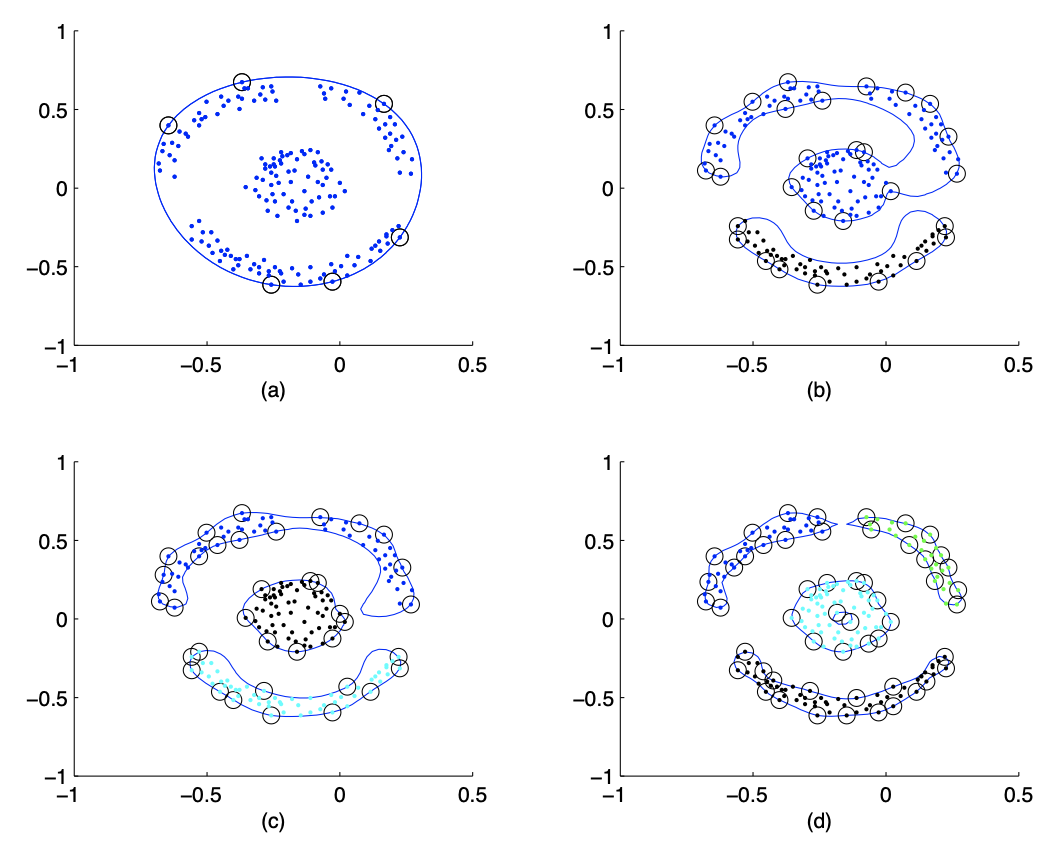
\includegraphics[scale = 0.75]{images/gaussian_kernel.png}
    \caption{Esempi di clusterizzazione con kernel gaussiano:
    q = 1 (b) q = 20 (c) q = 24 (d) q = 48 - da \cite{23}}
    \label{gaussian}
\end{figure}
\\
Quelli che seguono sono i tre vincoli del problema:
\begin{equation}\label{vincolo}
    \mu_i || \mathit{\Phi}(x_i) - a ||^2 \leq \mu_iR^2 + \xi_i \;,
\end{equation}
\begin{equation}\label{vincolo_2}
    (1 - \mu_i) || \mathit{\Phi}(x_i) - a ||^2 \geq (1 - \mu_i)R^2 + \tau_i \;,
\end{equation}
\begin{equation}\label{vincolo_3}
    \xi_i \geq 0, \tau_i \geq 0 \;.
\end{equation}
la soluzione originale viene, quindi, estesa minimizzando $R^2 + C\sum(\xi_i + \tau_i)$ tramite (\ref{vincolo}-\ref{vincolo_3}), dove $C$ è un iperparametro; la soluzione viene ricavata tramite un solver.
La fase successiva è di indurre il valore della funzione di appartenenza a tale insieme.

\subsection{Induzione di insiemi fuzzy}
Se $F$ è l'insieme fuzzy analizzato, l'algoritmo individua un suo sottoinsieme $K$, detto \textit{core}, in cui assegna l'unità come grado di appartenenza dei punti che ne fanno parte.
\\
Infine, sulla base del fuzzificatore impostato, l'algoritmo fa decrescere il valore man mano che i punti si allontanano dal core (Figura \ref{mulearnplot}). 
\begin{figure}
    \centering
    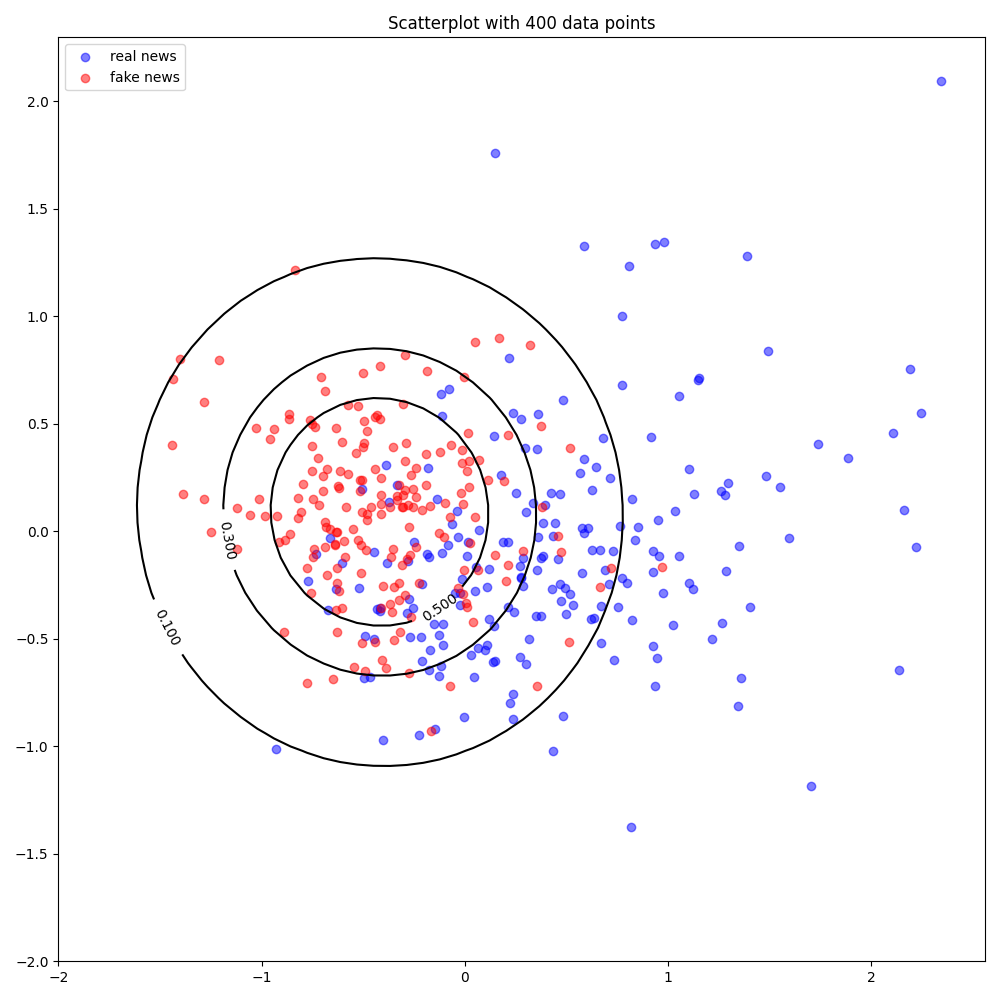
\includegraphics[scale=0.35]{images/mulearn.png}
    \caption{Visualizzazione in uno spazio bidimensionale dei punti (400 osservazioni) e del fuzzy set associato alle fake news indotto da $\mu$-learn. In rosso le notizie echitettate come ``fake'' e in blu come ``vere''.
    \\
    Le curve di livello discriminano le soglie dei gradi di appartenenza dei punti a partire dall'insieme core al centro fino al resto delle osservazioni nelle zone periferiche.}
    \label{mulearnplot}
\end{figure}
La fase di induzione della funzione di appartenenza è lo step in cui l'algoritmo viene effettivamente addestrato tramite i dati etichettati.
\\
L'esito dell'induzione della funzione di appartenenza è influenzato dalla scelta degli iperparametri.

\subsection{Iperparametri}
Gli \textit{iperparametri} sono parametri speciali che non vengono appresi direttamente dall'algoritmo di Machine Learning ma che sono fissati prima dell'addestramento.
Nel contesto considerato da questo elaborato si distinguono le seguenti quantità: 
\begin{enumerate}
    \item il solver utilizzato,
    \item il tipo di kernel,
    \item eventuali parametri che dipendono dal tipo di kernel,
    \item $C$,
    \item il tipo di fuzzificatore,
    \item eventuali parametri legati al tipo di fuzzificatore,
    
\end{enumerate}
Il primo è costituito da due possibilità: \textit{tensorflow} e \textit{gurobi}, due solver che usano strategie differenti per il problema di ottimizzazione non lineare; il secondo e il terzo condizionano la forma dell'insieme indotto, si pensi ad esempio a $\sigma$ per il kernel gaussiano, mostrato in precedenza.
\\
Il quarto impatta sulla dimensione del core dell'insieme:
all'aumentare di $C$, il core si dilata e incrementa il numero di elementi in esso inclusi.
Più precisamente, al raggiungimento dell'unità da parte di $C$ l'insieme fuzzy tende a un insieme regolare che racchiude i punti del campione le cui etichette sono diverse da zero.
\\
Infine, il quinto e il sesto sono legati al processo di fuzzificazione precedentemente definito nell'apposita Sezione.
Una volta prefissati gli iperparametri, è possibile ricorrere a una tecnica per la loro ottimizzazione, detta \textit{tuning}.

\paragraph{Tuning} Con tuning si intende l'addestramento di uno stimatore con diverse configurazioni dei suoi iperparametri, al fine di valutare i risultati delle predizioni e, sulla base di essi, scegliere opportunamente il set di valori ottimali per la generazione del modello finale.
\\
Concretamente, si può implementare il tuning tramite la cosiddetta \textit{grid search}: si tratta di una ricerca del modello migliore che considera una tabella di valori che si desidera esplorare ed è basata sulla \textit{cross validation}.

\paragraph{Cross validation} 
La cross validation è una tecnica che consiste nel partizionare il dataset in $k$ \textit{fold}, effettuare altrettante iterazioni e, per ciascuna, considerare l'$i$-esima fold come test set e le restanti $k-1$ come training set per addestrare il modello generato.
\\
In questo caso esistono diverse scuole di pensiero sulla percentuale che si preferisce impostare per la suddivisione in fold.
\\
Indirettamente, definire ogni combinazione delle fold equivale a definire un nuovo modello, pertanto fare una cross validation $k$-fold significa generare $k$ modelli.
\\
Questa tecnica ha il vantaggio di massimizzare l'utilizzo dei dati, evitando di costruire un validation set; inoltre, può essere usata per fare \textit{model selection} usando la sua versione ``innestata'': per ognuna delle iterazioni precedentemente descritte, si opera una cross validation interna per fare il tuning degli iperparametri e, dunque, generare $k$ modelli ottimizzati.
\\
Infine, questa tecnica rappresenta un metodo efficace per contrastare il problema di \textit{overfitting}, in quanto previene il fenomeno di \textit{data leakage}\footnote{Per data leakage si intende lo scenario in cui il training set viene contaminato dal test set. In altre parole violare la proprietà di disgiunzione tra questi due tipi di insiemi causa un eccessivo adattamento del modello sui dati di allenamento e, di conseguenza, performa molto bene su questi ultimi ma molto male su osservazioni nuove.}.

\paragraph{Overfitting e underfitting}
Essi rappresentano una buona frazione delle possibili insidie che si potrebbero incontrare durante l'addestramento di modelli predittivi.
\\
Gli iperparametri determinano i gradi di libertà del modello ottenuto; la loro numerosità, infatti, ha un impatto sulla complessità del modello: avere molti iperparametri rischia di complicarlo eccessivamente, dualmente averne pochi, lo rende potenzialmente troppo semplice. 
\\
Si distinguono, quindi, modelli che soffrono di underfitting quando hanno errore alto sul training set e sul test set, tipicamente questo è causato da un'eccessiva semplificazione del modello o una quantità di dati insufficiente.
\\
Al contrario, modelli che soffrono di overfitting sono troppo complessi e mostrano un errore basso sul training set ma alto sul test set, evidenziando una scarsa capacità di generalizzazione.
\\
In letteratura, il problema è descrivibile anche in termini di equilibrio tra \textit{bias} e \textit{variance error} \cite{31}: l'underfitting è il risultato del prevalere del bias error sul variance error; l'overfitting, invece, è causato dal dominare del variance error sul bias error.
\\
Di conseguenza, fare esclusivamente attenzione al problema di \textit{data leakage} non basta:
al fine di trovare un compromesso per controllare questo tipo di problematica, è necessario avere una giusta complessità del modello, associata a un campione di dati sufficientemente grande.

\section{Il sistema}
\label{sistema}
Nel presente Paragrafo si mostra ad alto livello l'architettura della soluzione proposta in questo elaborato, mostrando prima i nodi che la compongono e poi come sia stato utilizzato il modello $\mu$-learn nel contesto del riconoscimento delle fake news.
\\
Nella seconda parte viene, invece, descritto come i nodi in questione comunichino fra loro e quali file vengano generati durante l'utilizzo del sistema.
\\
Per gestire la pluralità dei casi nella forma dell'input, il sistema definisce un formato per i dataset che andrà a trattare: il dataset ideale è un dataframe che contiene in forma tabulare osservazioni relative a dati testuali che, nell'ambito trattato da questo elaborato, possono essere il corpo delle notizie o i titoli.
\\
Tali osservazioni sono etichettate con valore 1 se si tratta di una notizia fake, 0 altrimenti. L'obiettivo di $\mu$-learn sarà, quindi, indurre l'insieme fuzzy delle fake news.
\subsection{Architettura}
L'architettura del sistema è composta da tre nodi: il preprocessing del dataset, la selezione dei modelli migliori e la visualizzazione dei dati; segue, quindi, una breve descrizione di ciascun nodo più nel dettaglio.

\paragraph{Dataset preprocessing} All'inizio di questa fase ci sono tre possibili scenari: i) il dataset rispetta il formato, ii) il dataset è formattato diversamente e dunque necessita di una fase di rielaborazione per poter essere utilizzabile, iii) il dataset viene generato dal sistema stesso.
\\
In altre parole, nel secondo caso è necessario rendere la forma dell'input compatibile col formato predefinito; questo viene fatto da un modulo che ha la funzione di estrarre le informazioni fondamentali e di formare con esse il dataframe desiderato.
\\
A questo punto interviene la vera e propria fase di preprocessing che consiste nell'eseguire una pipeline di operazioni che hanno l'obiettivo di preparare il dataset alla fase successiva.
\\
Le operazioni in questione includono le tecniche di elaborazione del linguaggio naturale, descritte nel Capitolo \ref{Capitolo 1}.
\\
Tale pipeline viene opportunamente configurata a seconda delle esigenze per attivare o disattivare gli step per l'elaborazione dei dati, anche in base allo scenario considerato.
\\
Al termine del preprocessing, un nuovo dataset viene creato e scritto su file, per il suo utilizzo in un secondo momento. L'intero processo viene schematizzato in Figura \ref{preprocessmodule}.

\begin{figure}
    \centering
    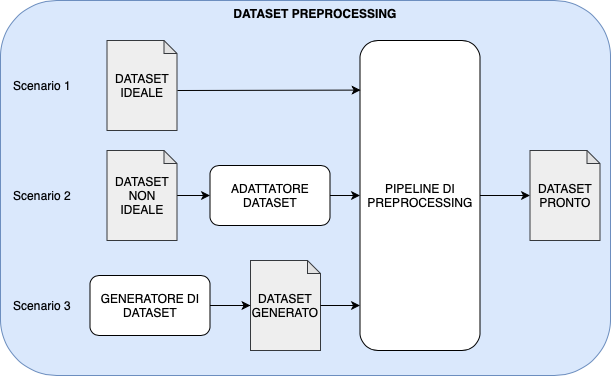
\includegraphics[scale=0.6]{images/preprocessingmodule.png}
    \caption{Primo nodo dell'architettura, il preprocessing dei dati, secondo i tre possibili scenari}
    \label{preprocessmodule}
\end{figure}

\paragraph{Model selection}
La fase di model selection si occupa di individuare il modello che meglio si adatta ai dati presi in esame.
\\
Al fine di rendere computazionalmente più agevole l'esecuzione e per ambire a risultati potenzialmente migliori, si applica la selezione a un dataset preprocessato.
\\
I modelli ottimali vengono generati tramite la tecnica della cross validation innestata e, per ciascuna iterazione, viene fatta una \textit{grid search} per indagare quali siano i migliori modelli sulla base del test error ottenuto.
\\
Alla fine di questa fase vengono ricavati, infatti, i modelli che si sono adattati meglio ai dati e fornita la relativa configurazione degli iperparametri.
\\
E' in questa fase che si colloca l'utilizzo di $\mu$-learn in quanto il test error concerne le predizioni dei modelli generati da $\mu$-learn.
I modelli selezionati vengono, dunque, serializzati per permettere il loro riutilizzo in un secondo momento; più precisamente, questo avviene nella fase di esperimenti in cui si vuole valutare il loro comportamento.
\\
In Figura \ref{selectionmodel} viene mostrata la rappresentazione del funzionamento sopra descritto.
\begin{figure}
    \centering
    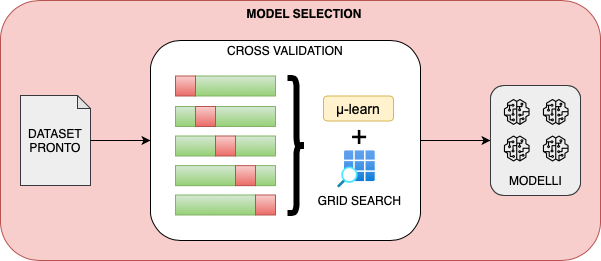
\includegraphics[scale=0.6]{images/modelselectionmodule.png}
    \caption{Secondo nodo dell'architettura, la selezione dei modelli}
    \label{selectionmodel}
\end{figure}

\paragraph{Data visualization} 
Nella parte di visualizzazione dei dati, i modelli vengono deserializzati per poterli riutilizzare e si opera un'analisi descrittiva.
\\
Tale analisi coinvolge principalmente i gradi di appartenenza approssimati dai modelli generati dal sistema, valutando la bontà delle predizioni da essi effettuate.
\\
Il criterio con cui viene valutata la correttezza delle predizioni consiste nell'utilizzare delle misure quantitative di errore. Queste metriche verranno approfondite nel dettaglio nel Capitolo \ref{Capitolo 3} ma, in generale, misurano il discostamento delle predizioni dalla \textit{ground truth}, ossia l'effettivo valore delle etichette nel dominio di conoscenza considerato, ad esempio 1 ("fake") e 0 ("vere") per le notizie.

\begin{figure}
    \centering
    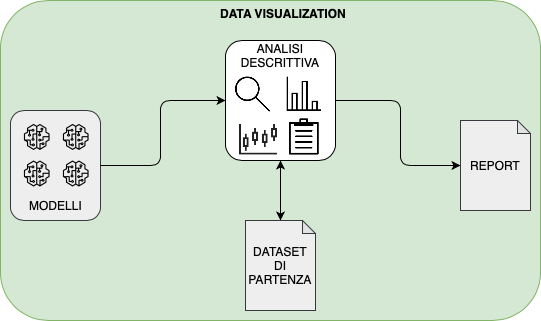
\includegraphics[scale=0.6]{images/datavisualizationmodule.png}
    \caption{Terzo nodo dell'architettura, la visualizzazione dei dati}
    \label{datavisualization}
\end{figure}

\subsection{Funzionamento del sistema}
In questo Paragrafo si descrive come funziona il sistema nella sua complessità e come esso sia stato utilizzato per produrre dei risultati.
\begin{figure}[!ht]
    \centering
    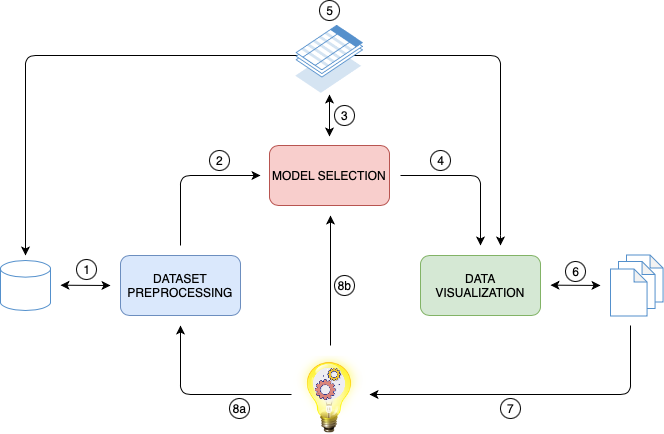
\includegraphics[scale=0.6]{images/cycle.png}
    \caption{Schema del flusso di comunicazione all'interno del sistema}
    \label{cycle}
\end{figure}
\\
In Figura \ref{cycle} viene raffigurato il flusso di comunicazione all'interno del sistema, numerato passo per passo: 
\begin{enumerate}
    \item il processo ha inizio quando si dispone di un dataset, ottenuto in uno dei modi visti in precedenza, e viene così acquisito dal primo nodo per il preprocessing;
    \item  il nodo ha prodotto un nuovo dataset rielaborato e pronto per l'addestramento. Ogni dataset preprocessato viene opportunamente scritto su file per permettere la successiva lettura;
    \item i modelli predittivi ottimali sono stati trovati, serializzati e il sistema aggiorna la storia degli esperimenti, documentata in un registro dedicato. Lo scopo del registro è catalogare i modelli e i loro dati associati tramite l'informazione di data e ora;
    \item i modelli vengono deserializzati e usati per l'analisi descrittiva delle predizioni;
    \item tramite il registro, il sistema è in grado di risalire al dataset utilizzato per ottenere i relativi modelli e, dunque, completare l'analisi;
    \item il modulo per la visualizzazione dei dati fornisce un report che viene aggiunto a quelli associati agli altri esperimenti;
    \item il report permette di analizzare il comportamento dei modelli, di individuare eventuali fonti d'errore e correggere la configurazione del sistema;
    \item a) la causa di errore è localizzata nel preprocessing dei dati e dunque è necessario ricominciare l'esperimento dall'inizio, andando a modificare i parametri in questione;
    \\
    b) la causa di errore riguarda il modo in cui viene fatta la grid search, pertanto si modifica i relativi valori a partire dalla model selection.
\end{enumerate}

\chapter{Implementazione}
\label{Capitolo 3}
\onehalfspacing
Il Capitolo \ref{Capitolo 3} tratta l'implementazione della soluzione proposta in precedenza.
\\
All'interno del Paragrafo \ref{pipeline} viene illustrata la pipeline di preprocessing, il Paragrafo \ref{modelselection} descrive la fase di model selection, mentre il Paragrafo \ref{evaluation} definisce i punteggi utilizzati per misurare la bontà dei modelli selezionati.

\section{Pipeline di preprocessing}\label{pipeline}
Per la fase di preprocessing è stata predisposta una pipeline, ovvero un insieme di operazioni eseguite consecutivamente.
\\
La sequenza di operazioni viene configurata al momento dell'esecuzione tramite un'opportuna parametrizzazione degli step della pipeline.
\\
Ogni operazione segue il pattern di implementazione della libreria \textit{scikit-learn}, che prevede di separare le procedure di \textit{fit}, \textit{predict} e \textit{transform}.
\\
Nel caso di operazioni di rielaborazione dai dati, vengono prese in considerazione \textit{fit} e \textit{transform} che definiscono rispettivamente la parte di apprendimento dei dati, quando richiesta, e quella di effettiva trasformazione dell'input in un output processato.
\\
Adottare questa convenzione rappresenta un vantaggio per poter accedere alle funzioni della libreria menzionata sopra, utilizzando ad esempio la pipeline stessa direttamente come parametro.
Inoltre, il codice organizzato in questa maniera si presta bene a future estensioni e favorisce la sua manutenibilità poiché rispetta il criterio della \textit{Separation of Concerns}, concetto chiave nell'ambito dell'Ingegneria del software \cite{32}.
\\
Quella che segue è la lista dei parametri della pipeline che al momento della configurazione è possibile attivare a seconda delle esigenze:
\begin{itemize}
    \item Lowercase,
    \item Rimozione dei duplicati,
    \item Tokenizzazione,
    \item Lemmatizzazione,
    \item Stemming,
    \item Rimozione del rumore,
    \item Rimozione delle stop word,
    \item Word2Vec,
    \item Aggregazione,
    \item Doc2Vec.
\end{itemize}
Intuitivamente, le operazioni non sono tutte compatibili, al contrario, alcune sono tra di loro esclusive, come Word2Vec e Doc2Vec, oppure la lemmatizzazione e lo stemming.
Inoltre, l'ordine con cui esse vengono applicate è determinante per la rielaborazione del testo: è più semplice rimuovere il rumore analizzando i token piuttosto che le stringhe di intere frasi, ecco perchè la tokenizzazione avviene tipicamente all'inizio della pipeline.\\
Infine, alcune operazioni possono escluderne delle altre: l'aggregazione, ad esempio, è necessaria solo in caso di utilizzo di Word2Vec.

\begin{figure}
    \centering
    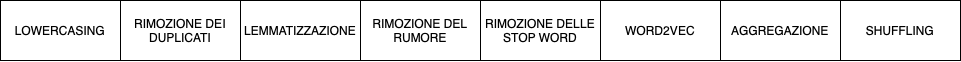
\includegraphics[scale=0.5]{images/pipeline.png}
    \caption{Esempio di configurazione di una pipeline di preprocessing}
    \label{pipeline}
\end{figure}

In Figura \ref{pipeline} viene mostrato un esempio di pipeline che è stata frequentemente utilizzata durante gli esperimenti.
\\
Si noti come in questo tipo di configurazione non sia necessario includere lo step di tokenizzazione in quanto la lemmatizzazione prevede una suddivisione in token che garantisce lo stesso risultato.

\subsection{Lowercasing}
Il \textit{lowercasing} è una tecnica che consiste nel trasformare una stringa di testo in una stringa composta unicamente da caratteri minuscoli.
\\
\\
\textbf{Input}: stringa, ``\textit{As of Tuesday evening, more than 8,000 hectares (nearly 20,000 acres) had been burned and hundreds of firefighters were involved in controlling the fire, according to DFES. The department said the cause of the 'out-of-control' blaze is unknown.}''
\\
\textbf{Output}: stringa, ``\textit{as of tuesday evening, more than 8,000 hectares (nearly 20,000 acres) had been burned and hundreds of firefighters were involved in controlling the fire, according to dfes. the department said the cause of the 'out-of-control' blaze is unknown.}''

\subsection{Rimozione dei duplicati}

\subsection{Rimozione del rumore}
\subsection{Lemmatizzazione}
\subsection{Rimozione delle stop word}
\subsection{Word2Vec}
\subsection{Aggregazione}
\section{Selezione dei modelli}\label{modelselection}
\subsection{Tuning degli iperparametri}
\subsection{Cross validation}
\subsection{Grid search}
\section{Valutazione dei modelli}\label{evaluation}
\subsection{Matrice di confusione}
\subsection{Precision, Recall e F1}

\chapter{Valutazione sperimentale}
\label{Capitolo 4}
\onehalfspacing
\section{Dataset}
\subsection{Dataset Kaggle}
\subsection{Campione}
\subsubsection{Estrazione del campione}
\section{Esperimenti}
\subsection{Analisi descrittiva}
\subsection{Curve di livello}
\subsection{Performances dei modelli}
\subsection{Baseline}
\subsection{Confronto dei modelli vs baseline}
\section{Vantaggi dell'approccio proposto}
\subsection{Classe di indecisione}
\subsection{Modello LDA}
\subsection{Approssimazione delle membership}

\chapter*{Conclusioni e sviluppi futuri}
\addcontentsline{toc}{chapter}{Conclusioni e sviluppi futuri}
\markboth{Conclusioni e sviluppi futuri}{} 
\onehalfspacing

Integrare l'analisi delle fake news con tecniche di image e video processing per modellare il problema più complesso in cui anche immagini e video svolgono un ruolo centrale nelle fake news (es: immagini vecchie riusate per notizie nuove, video che non corrispondono ai fatti riportati).

\printbibliography

%			RINGRAZIAMENTI
%
\prefacesection{Ringraziamenti}

\end{document}



